\documentclass[a4paper]{article}

\usepackage[english]{babel}
\usepackage[utf8]{inputenc}
\usepackage{amsmath}
\usepackage{graphicx}
\usepackage[colorinlistoftodos]{todonotes}
\usepackage{array}
\usepackage{hyperref}

\title{Technical Specifications}

\author{Joel Hutton}

\date{February 6th 2016}

\begin{document}
\maketitle
\section{Hardware}

\subsection{Wheelbase}
\subsubsection{Dimensions}
'Drive' wheelbase:		15cm \newline
Radius of 'turn' wheel: 11cm
\subsubsection{Origin}
The origin is directly between the 'Drive' wheels
\subsubsection{Arrangement}
The robot uses a 3 wheeled 'T' design with 2 parallel 'drive' wheels along one axis of rotation (capable of rotating independently) and a third unpowered 'turn' wheel rotating perpendicular to these 2 (figure 2). The 'origin' of the robot should be 
directly between the 2 drive wheels which are 15cm apart. The 'turn' wheel 
is 11cm back from the origin, the left wheel 7.5cm to the left and the right
7.5cm to the right. 

\subsubsection{Motors}
The 2 drive motors are lego NXT motors and have rotational encoders built in, this is used to turn and move accurately. 
\subsubsection{Wheels}
The wheels at the left and right are large 80mm in diameter ribbed rubber wheels. The wheel at the rear is a large holonomic wheel 64mm in diameter
\subsubsection{Performance}
The performance was measured through the rotary encoders to be:\\
max acceleration(stable):$2.5ms^{-2}$\\
max speed(stable):$1ms^{-1}$ \\
max deceleration (hard brake):$20ms^{-2}$\\
see Figure 1 for profiling\\

\subsubsection{Chargeable Parts and Costs}
\begin{center}
\begin{tabular}{ | m{3cm} | m{3cm}| m{6cm} | }
\hline
\textbf{Part} & \textbf{Quantity} & \textbf{Total Cost} \\
\hline
holonomic wheel & 1 & £6 \\
\hline
NXT motor       & 2 & £5 \\
\hline
\textbf{total} & \textbf{3} & £16 \\
\hline
\end{tabular}
\end{center}


\begin{figure}[!ht]
\caption{speed time profiling}
\centering
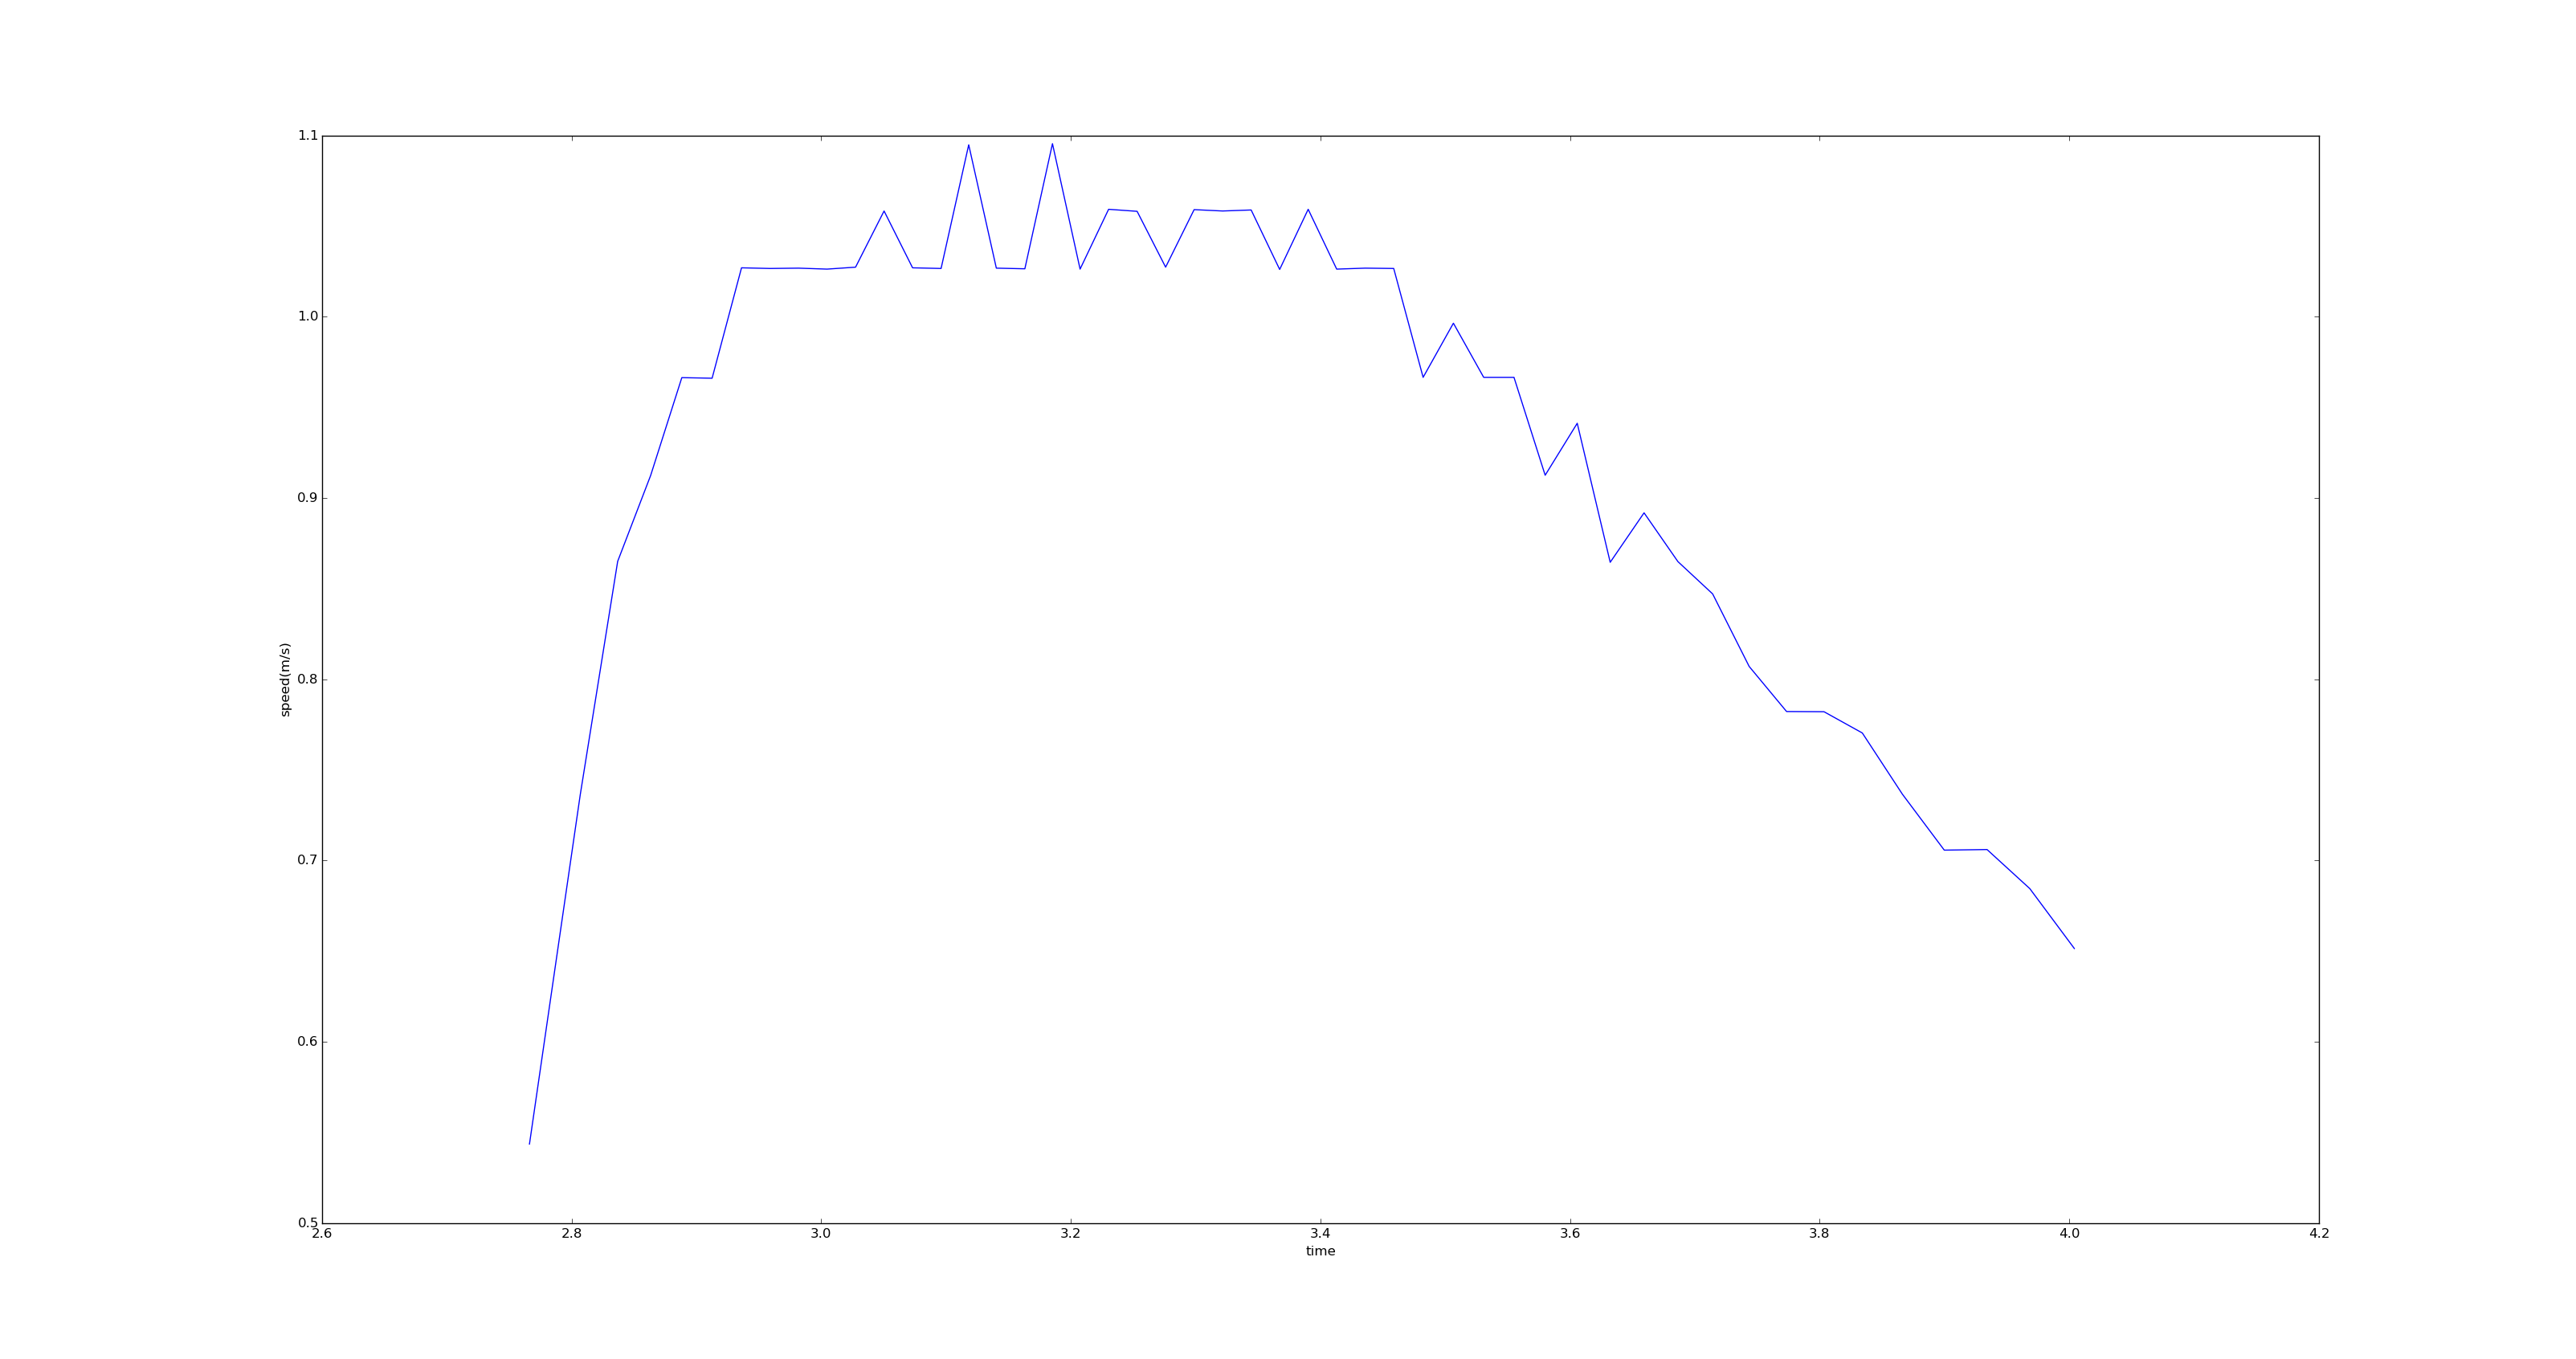
\includegraphics[width=\textwidth, angle=0]{speed_time_ms.png}
\end{figure}
\begin{figure}[!ht]
\caption{wheels as viewed from rear}
\centering
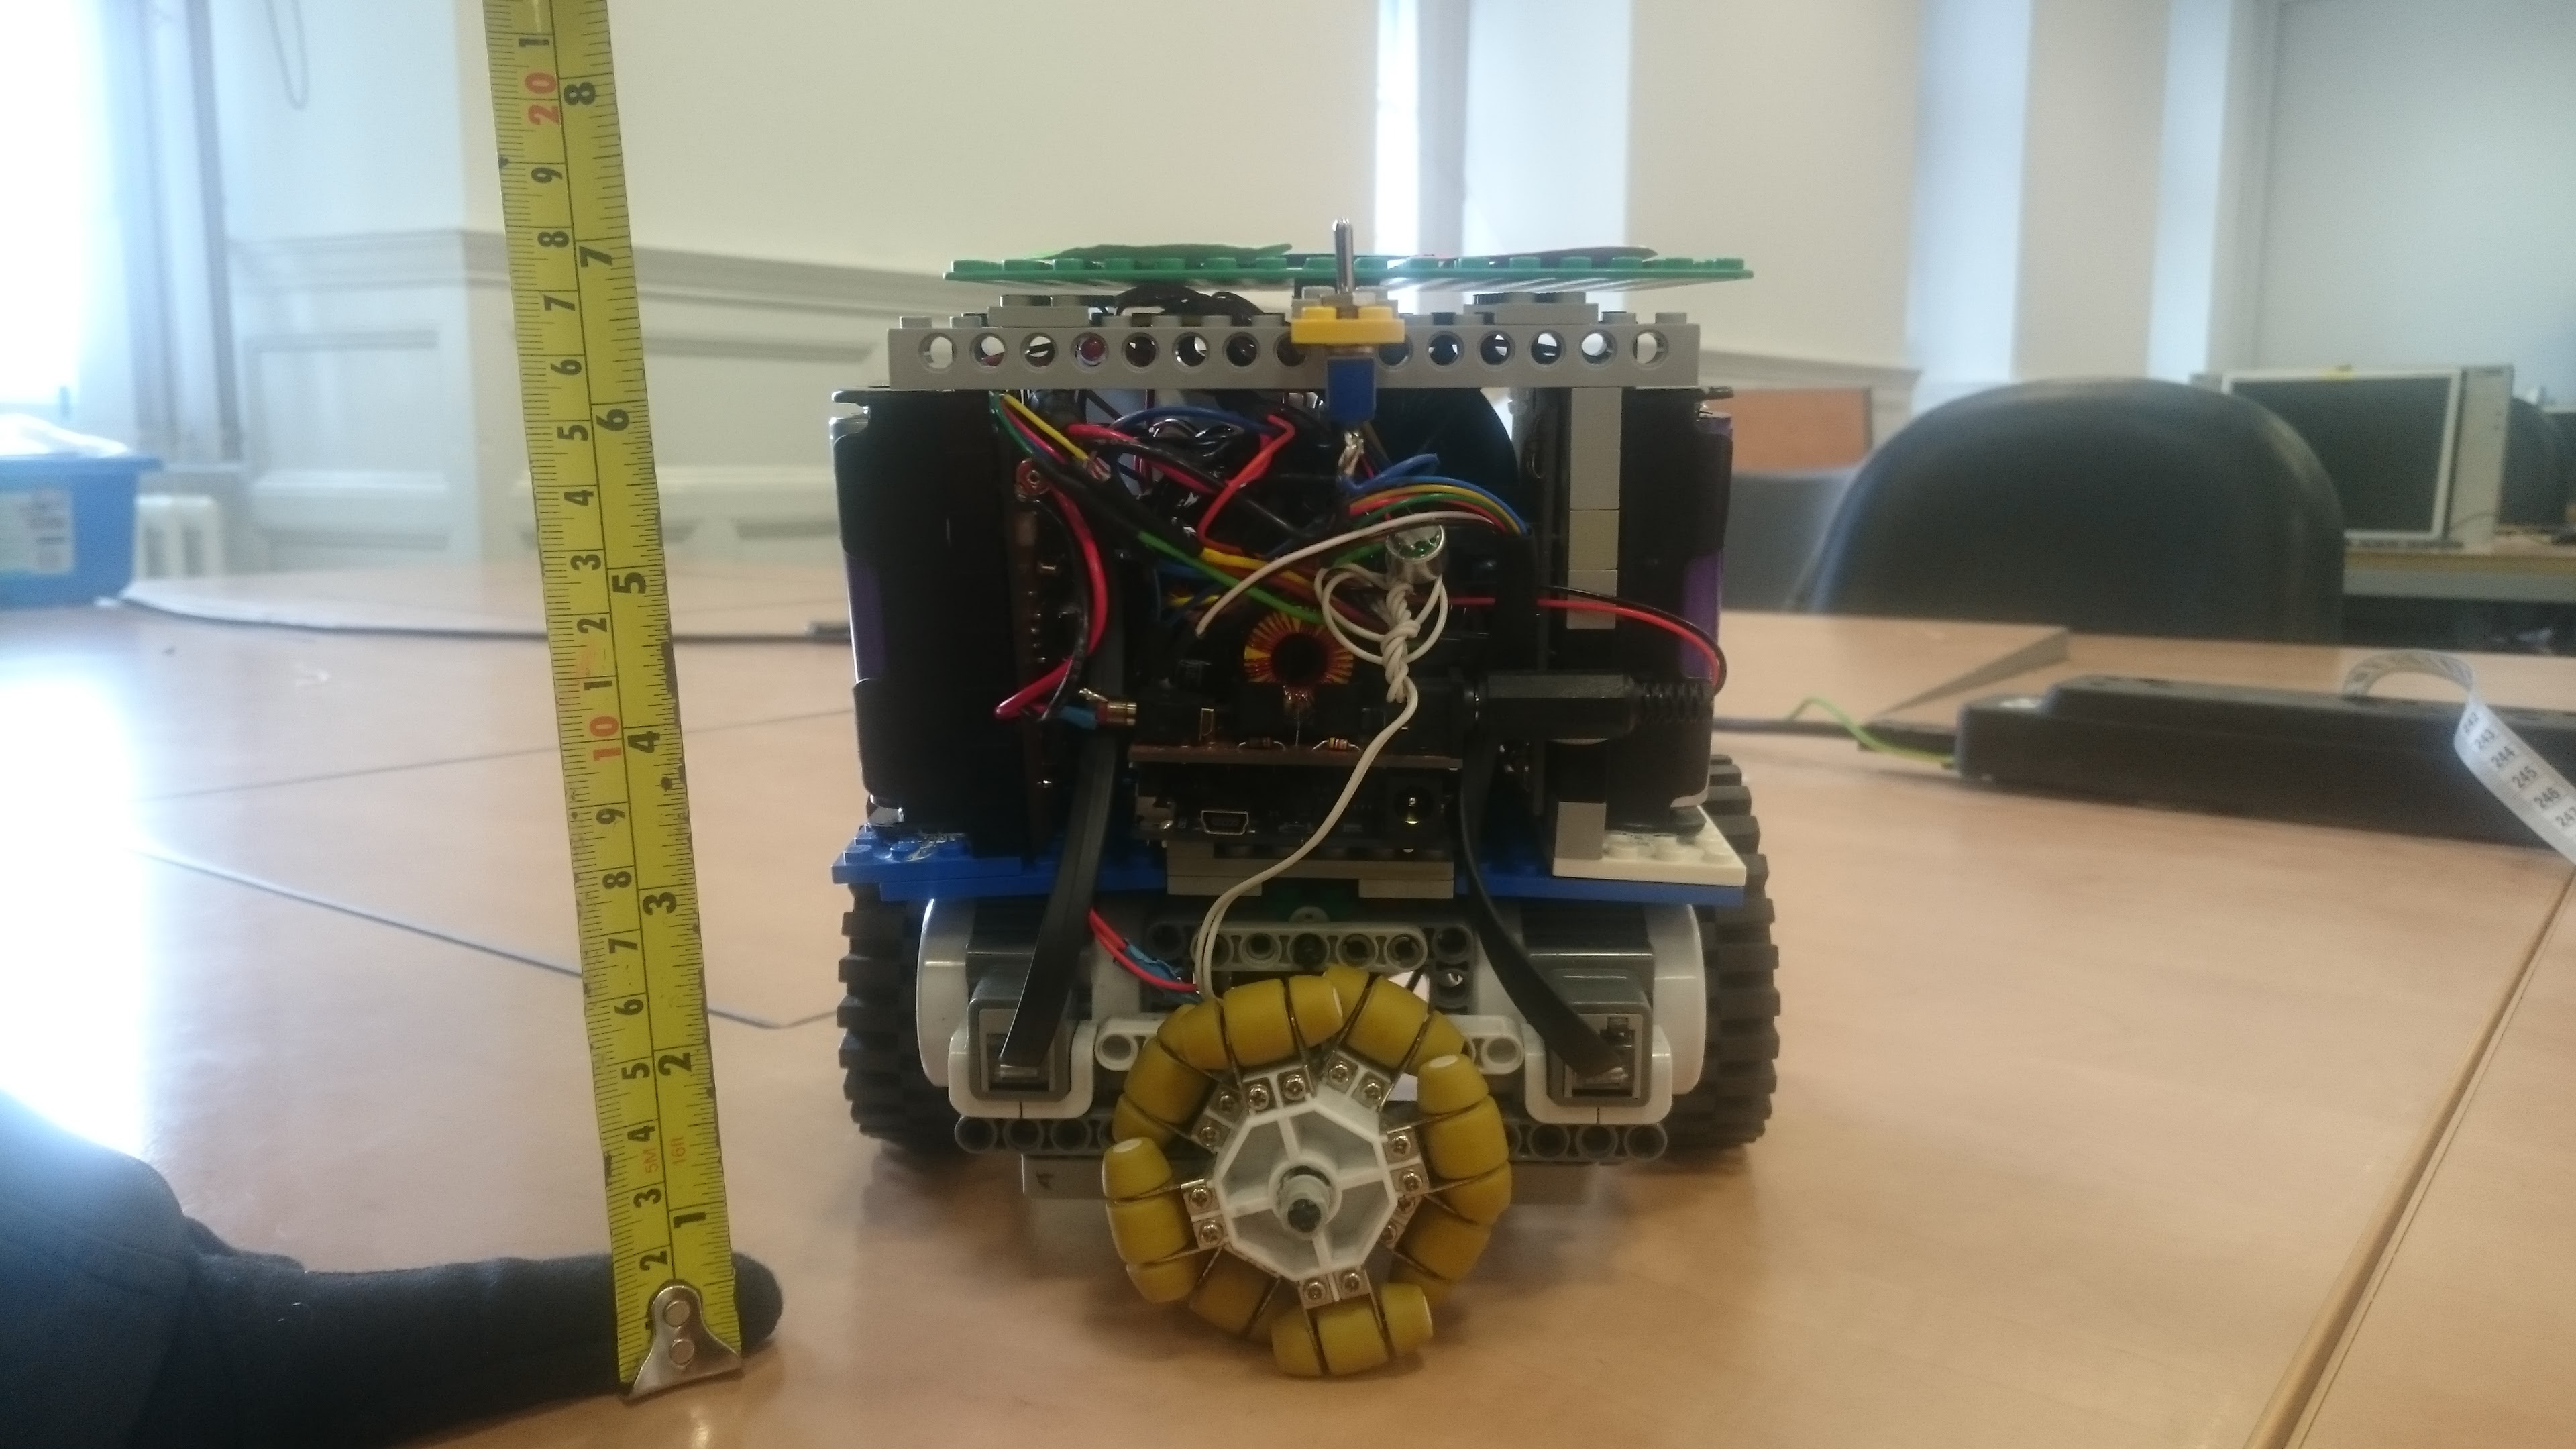
\includegraphics[width=\textwidth, angle=0]{DSC_0151.jpg}
\end{figure}

\subsection{Design Decisions}
The 3 wheeled design was chosen for simplicity and accuracy. The robot does not need to strafe as it is an offensive robot and does not defend the goal, it approaches the ball head on and it shoots head on. The 3 wheeled design requires only 2 motors, which is power efficient, and makes the turning and moving software simple. The 3rd wheel was initially powered but it caused the robot to turn inaccurately as it was difficult to precisely match the speeds of the 3 motors. The 'T' shape made forward movement and mounting the grabbers trivial and gave plenty of room to mount a kicker underneath. Having both powered wheels facing directly in the direction of primary movement gave excellent acceleration and speed.

\subsection{Front Assembly}
\subsubsection{Description}
The robot Has a 2 motor assembly mounted on 4 vertical bars coming up from the struts joining the left and right NXT drive motors. These are symmetrically mounted and linked by a chain in order to keep them synchronised. The right grabber is lower than the left one so that they do not hit into each other. On one of the centre axles there is a rotary encoder to give the position of the grabbers to the arduino, through the rotary encoder board. This allows the grabbers to be opened to a point where they do not hit the wheels, maintain a closed position without constant current and detect when the grabbers will not fully close, implying there is a ball in the way. There is an ultrasound module for automatically avoiding collisions mounted between the motors. 

The grabber assembly is fully detachable and can be clipped on and off. 
\begin{figure}[!ht]
\caption{front assembly}
\centering
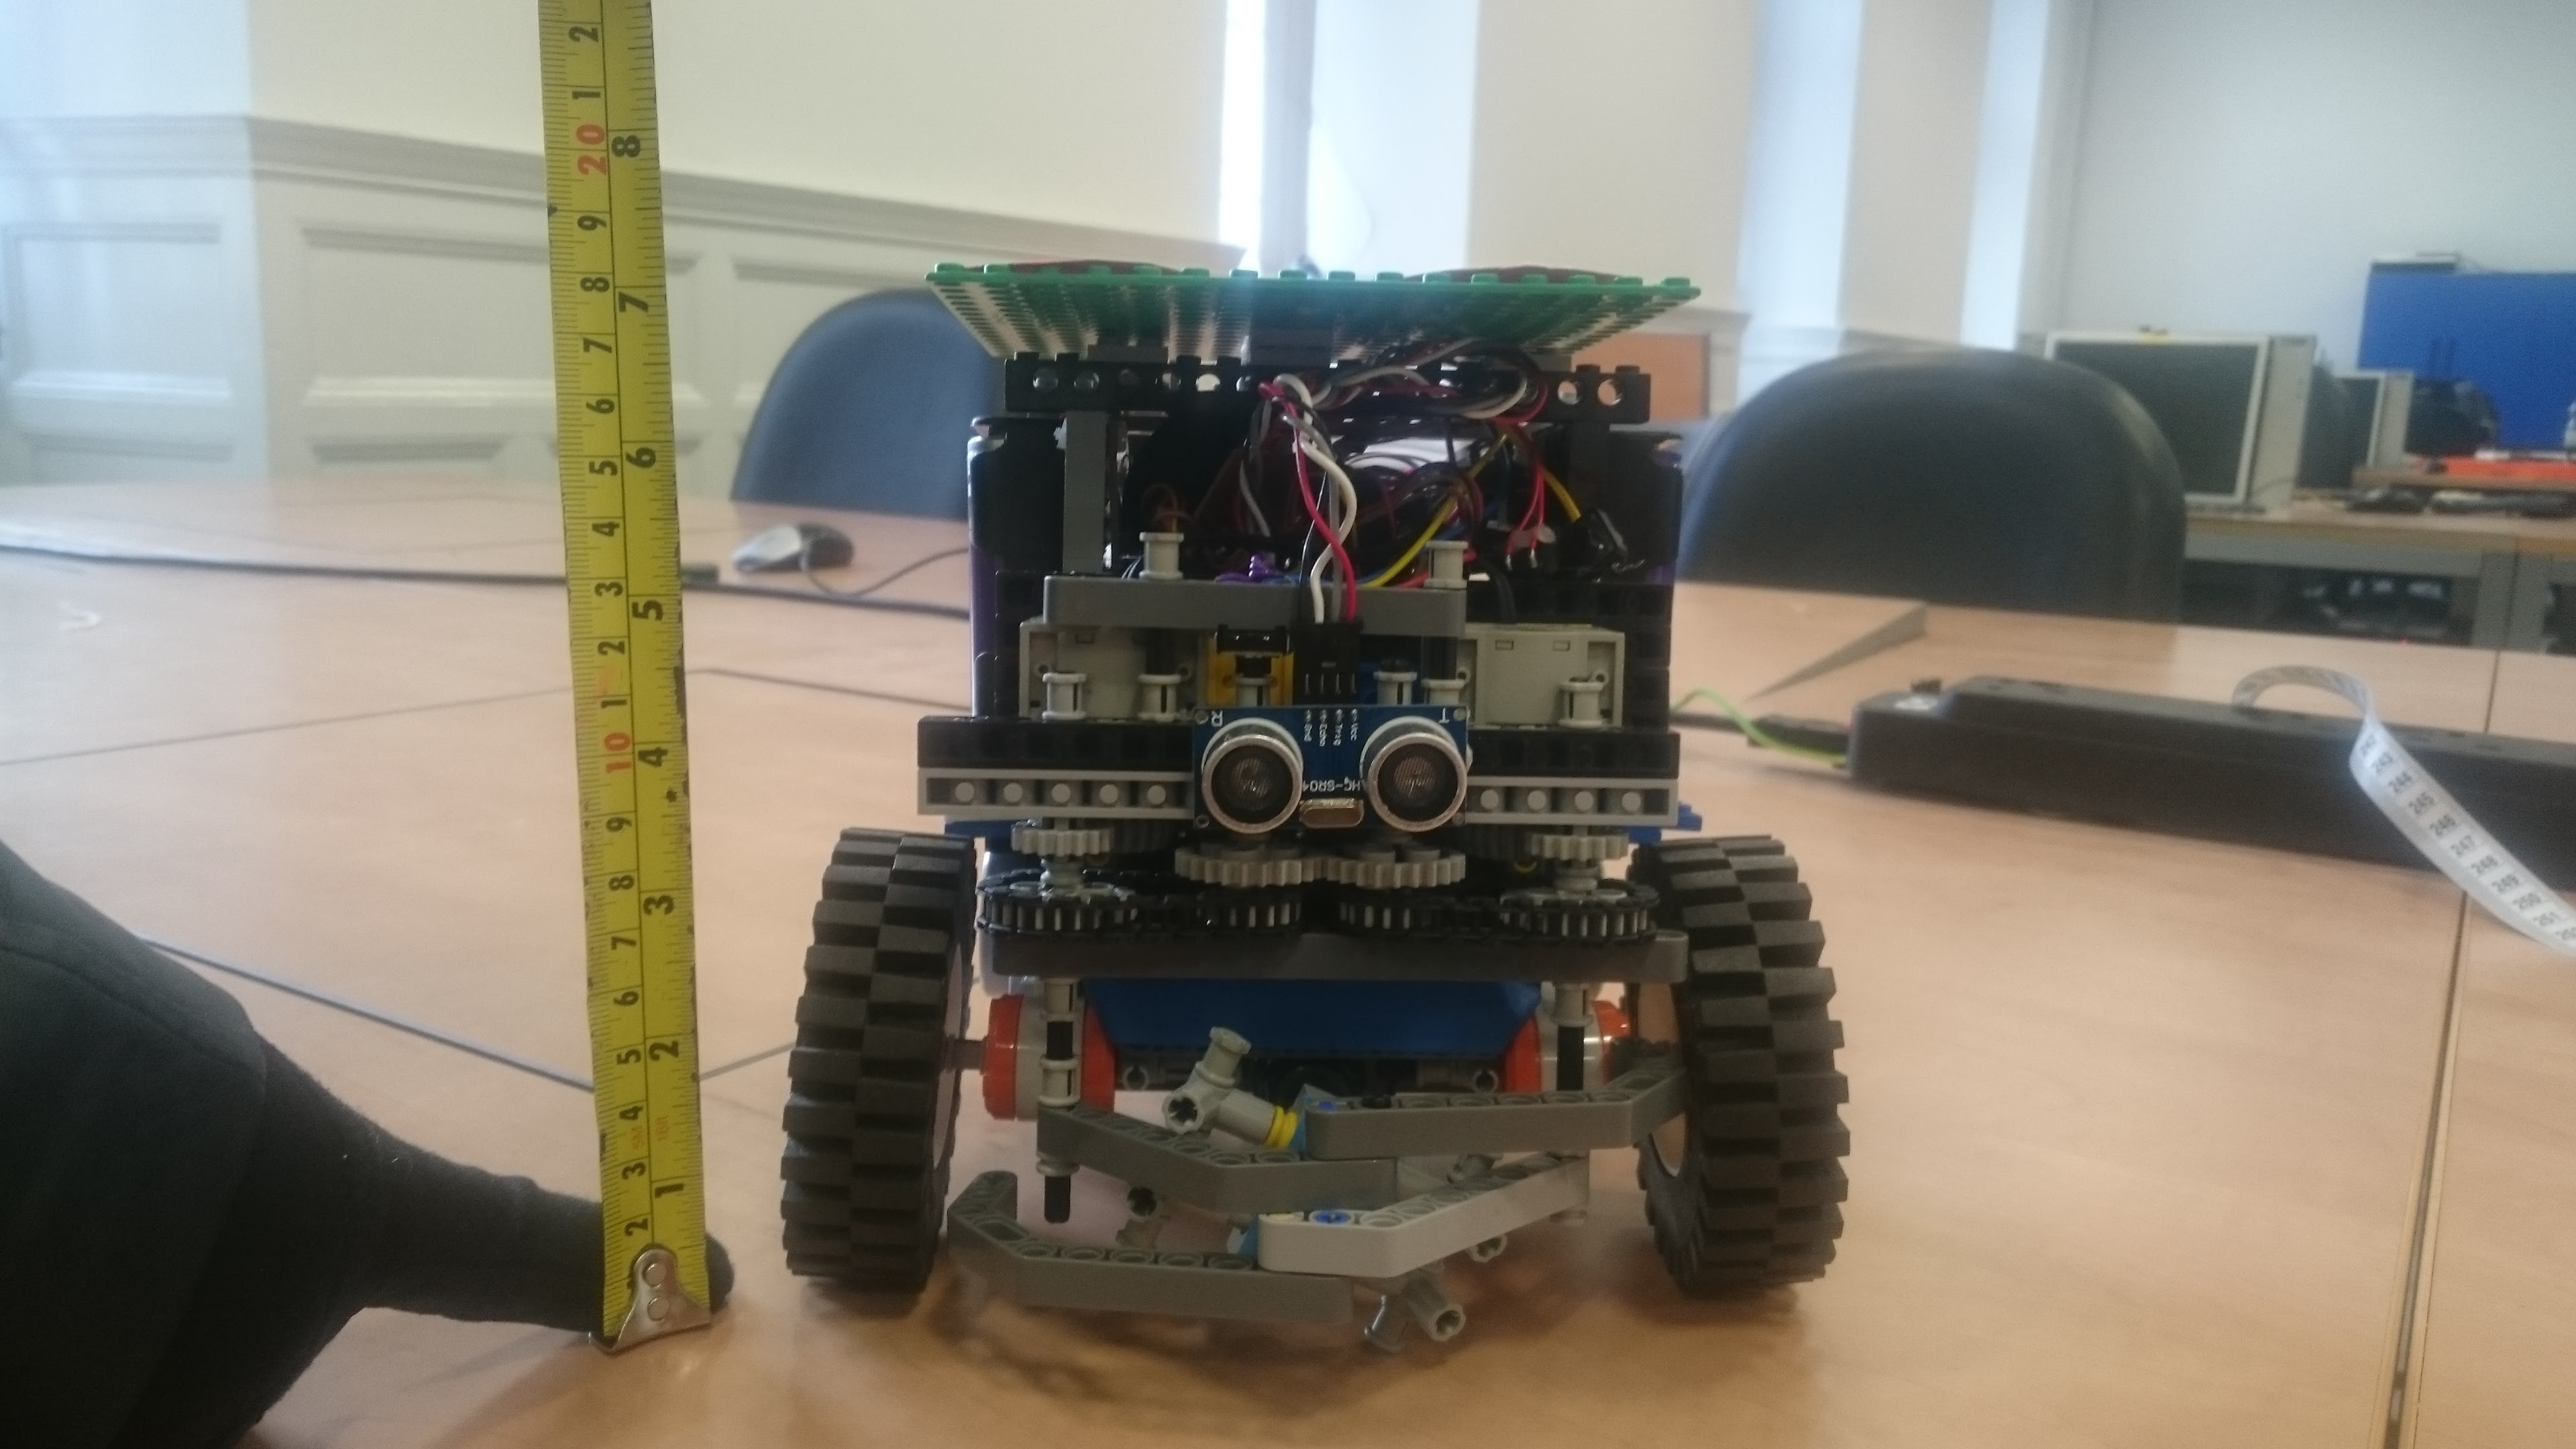
\includegraphics[width=\textwidth]{DSC_0149.jpg}
\end{figure}

\subsubsection{Parts and Costs}

\begin{center}
\begin{tabular}{ | m{3cm} | m{3cm}| m{6cm} | }
\hline
\textbf{Part} & \textbf{Quantity} & \textbf{Total Cost} \\
\hline
43362 Electric Technic Mini-Motor 9v & 2 & £1 \\
\hline
Ultrasound Module       & 1 & £2.60 [2]\\
\hline
\textbf{total} & \textbf{3} & £3.60 \\
\hline
\end{tabular}
\end{center}

\subsubsection{Design Decisions}
The motors were chosen as the shape of them provided good structure for strong mounting. It was decided to use 2 for symmetrical weight distribution. The chain was added after it was found the grabber touching the ball was usually slower and could cause the mechanism to jam when one grabber closed faster.
\\ \\
The rotary encoder was added when it was found to be exceptionally difficult to determine if the ball was in the grabbers, as well as exceptionally difficult to prevent the grabbers hitting the wheels. An added benefit was that the grabbers could keep the ball without a constant current, by powering on if they opened beyond a threshold during movement. 

\subsection{Kicker}
\begin{figure}[!ht]
\caption{Underside of Robot With Previous Wheels}
\centering
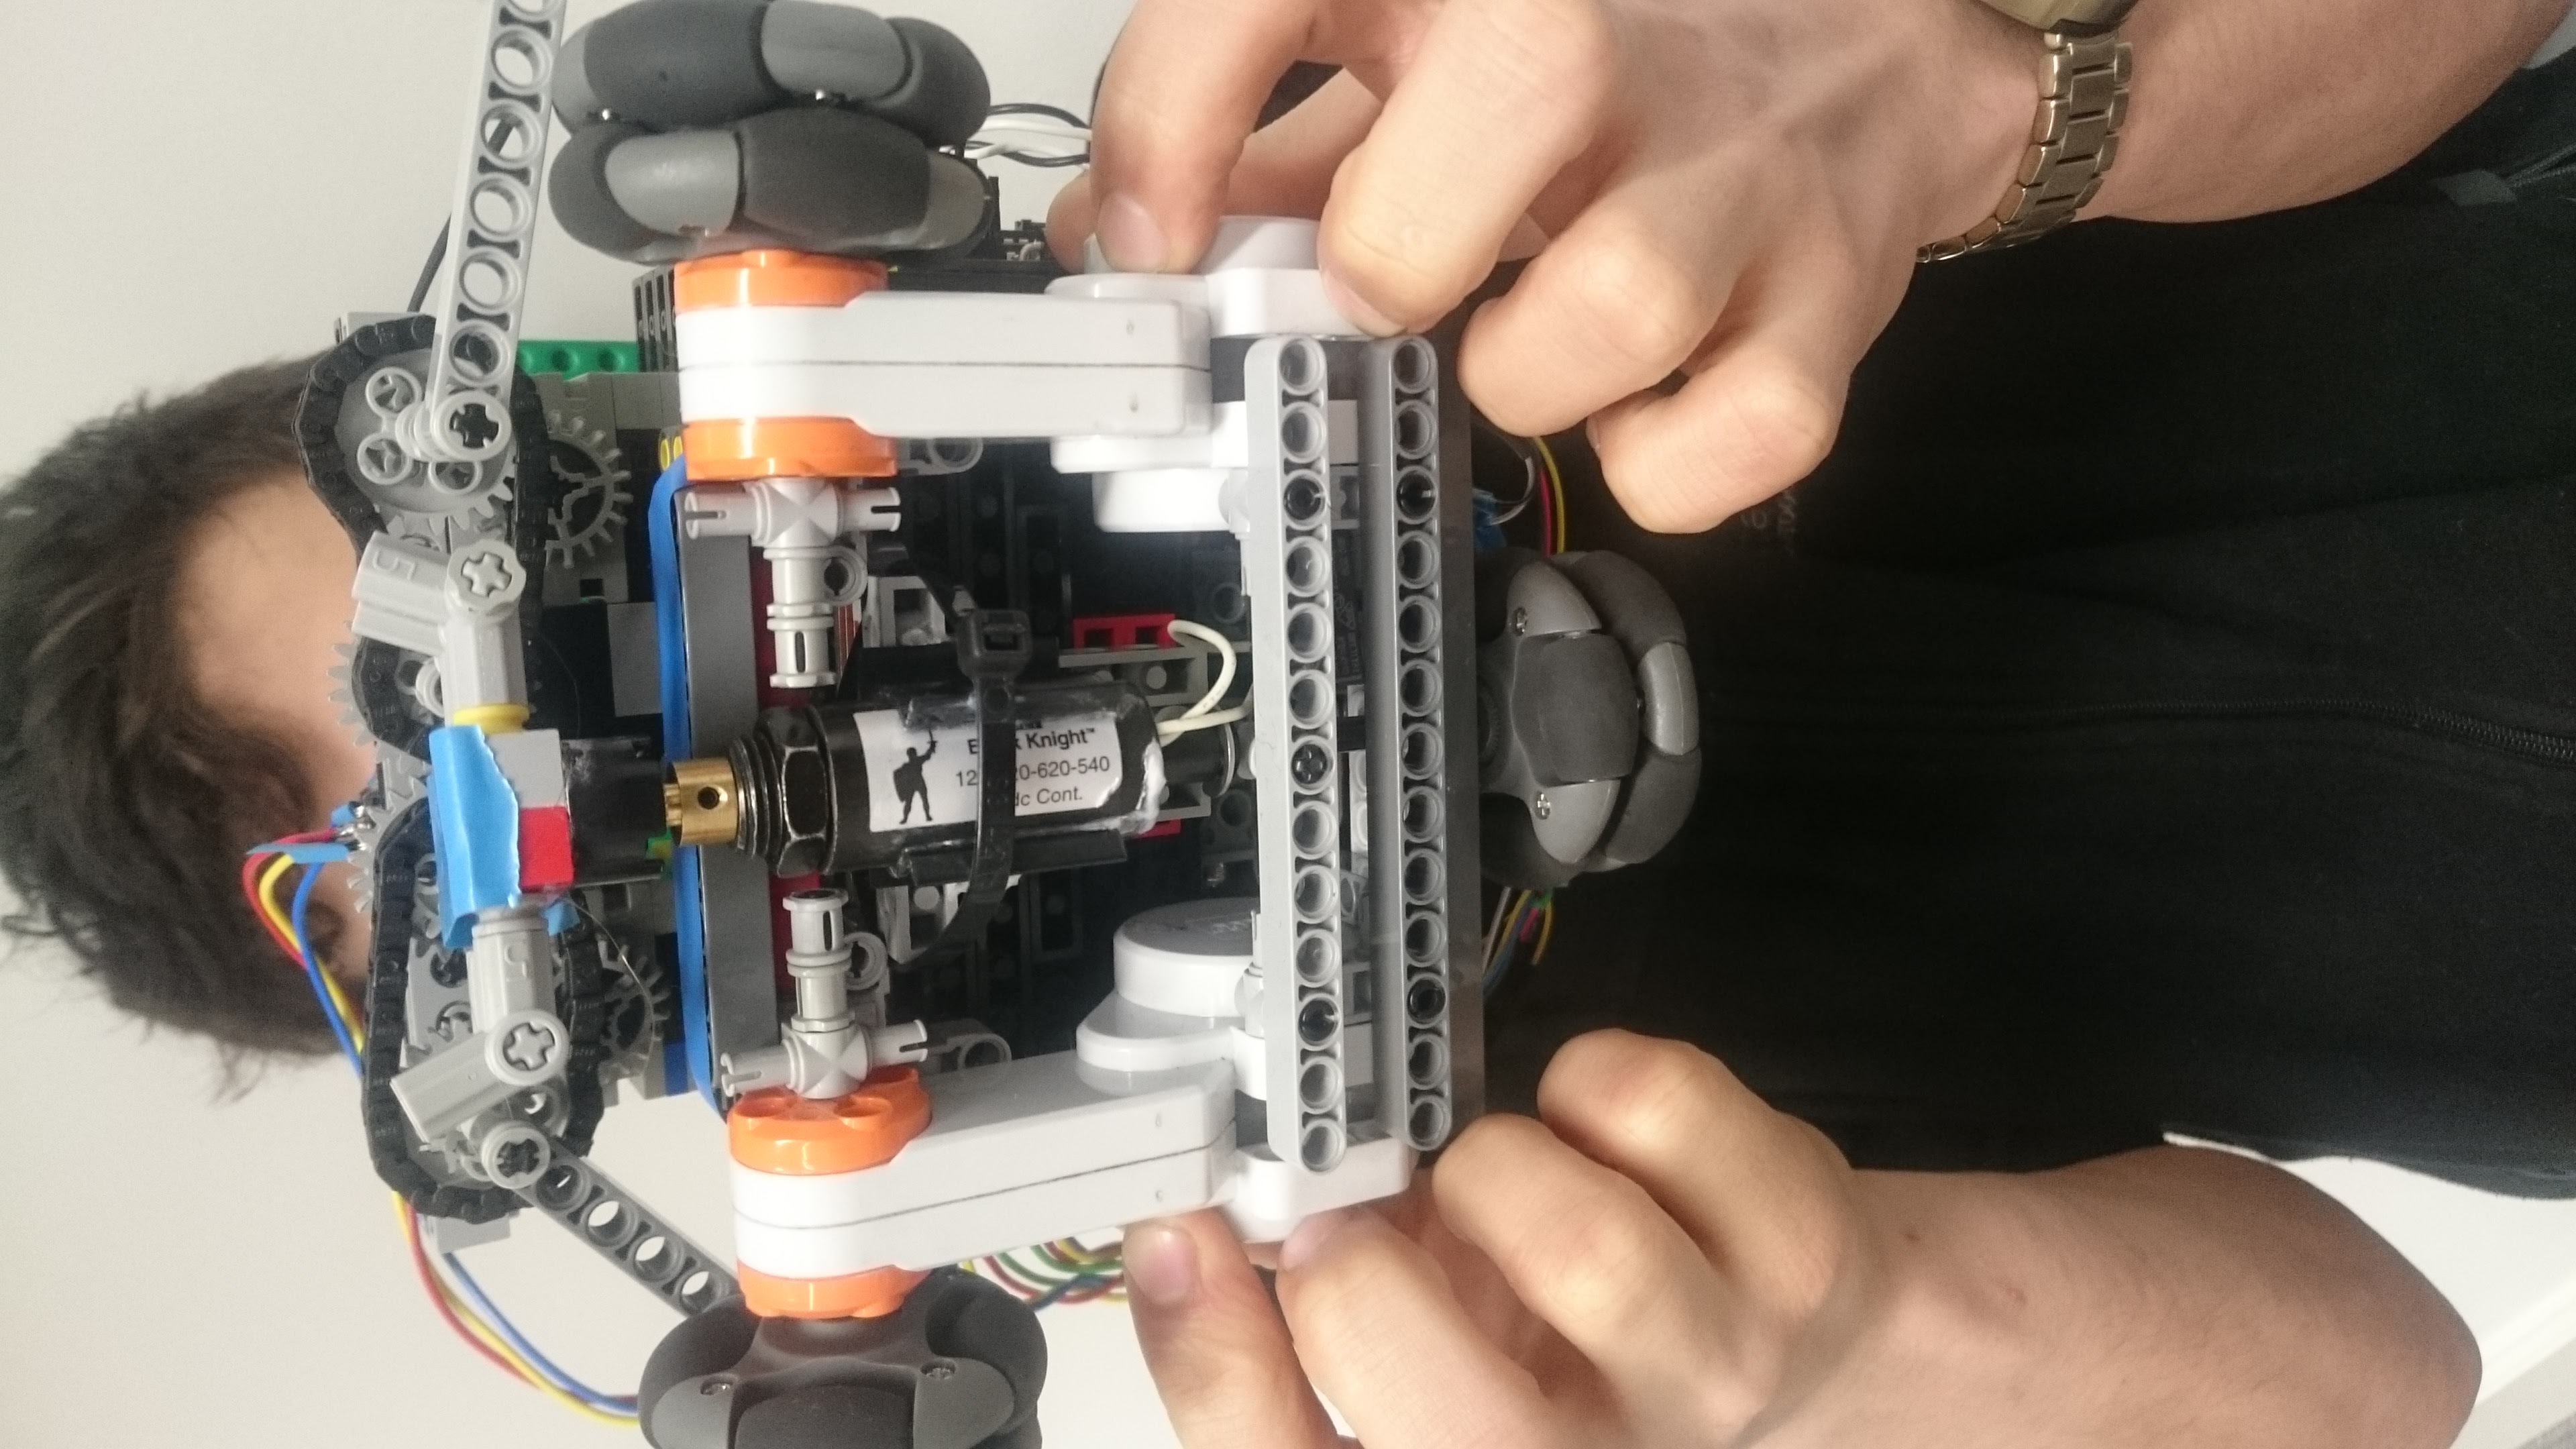
\includegraphics[width=\textwidth, angle=270]{DSC_0036.jpg}
\end{figure}
\subsubsection{Position}
The kicker is a solenoid mounted on the underside of the robot (see Figure 4) connected through a relay to the battery packs, with the relay signal going to the power regulator board and being controlled directly by the arduino. On the end of the solenoid is a curved piece of lego designed to keep the ball straight as it pushes it.

\subsubsection{Performance}
Max distance: 3.2m 
Max error (radius of target):15\%

\subsubsection{Parts and costs}
\begin{center}
\begin{tabular}{ | m{3cm} | m{3cm}| m{6cm} | }
\hline
\textbf{Part} & \textbf{Quantity} & \textbf{Total Cost} \\
\hline
121-420-610-540  SOLENOID, 6V & 2 &  £10.91[1] \\
\hline
769-JQ1A-5V-F Relay & 1 &  £2.80[2] \\
\hline
\textbf{total} & \textbf{3} & £13.71 \\
\hline
\end{tabular}
\end{center}

\subsubsection{Design Decisions}
The solenoid kicker was chosen as it took up little space, was reliable and was powerful. With the saving in space longer grabbers could be fitted, making grabbing more reliable. Due to unreliable performance and a lack of space a previous design using motors to drive a kicker was abandoned.

\subsection{Board and Battery Assembly}
\subsubsection{Structure}
The boards are mounted on a platform in the middle of the 3 wheels. The arduino and power
shield are mounted in the centre with 2 battery packs of 2 18650 Li-Ion batteries mounted sideways on either side. The rotary encoder board is
mounted on the back of the right battery pack and the motor driver board is mounted
on the left battery pack. All wires are kept on the inside of the robot.

\subsubsection{Batteries}
The batteries are 4* 18650 Canwelum Li-Ion cells wired in series in 2 battery packs. They can be removed and charged individually in the Li-Ion charger.
	Voltage (per cell):2.65V(min), 3.7(nominal) 4.2V(max)
    Voltage (total)   :10.6V(min), 14.8V(nominal), 16.8V(max)
    Max Current: 7A
    Internal Resistance (per cell): 0.150 Ohms
    Internal Resistance (total)   : 0.6   Ohms
    Capacity: 2250mAh
	Protection: overvolt and undervolt   
    
\subsubsection{Connections}
The batteries are connected in series and power the regulator board, which regulates the voltage to the motors and arduino. The kicker solenoid is powered directly from the power pack. The relay powering the kicker is connected to the arduino pin 6 and ground. The motor and encoder boards are connected to the power shield by I2C wires. 
\subsubsection{Switch}
A yellow switch turns power from the power packs to all parts of the robot on and off.

\subsubsection{Parts and costs}
\begin{center}
\begin{tabular}{ | m{3cm} | m{3cm}| m{6cm} | }
\hline
\textbf{Part} & \textbf{Quantity} & \textbf{Total Cost} \\
\hline
Canwelum 18650 protected Li Ion cells & 8 &  £40[4] \\
\hline
Nitecore Charger & 1 & £14.99 [6]\\
\hline
Battery Holder & 2 & £3.88 [5]\\
\hline
\textbf{total} & \textbf{3} & £58.87 \\
\hline
\end{tabular}
\end{center}

\subsection{Design Decisions}
The design was subject to much revision, and was changed after encountering specific problems. It was decided to add a switch after trouble stopping the robot when it was out of control, this also helps preserve battery life when not in use. The rotary encoder board and motor board were initially facing out to give easy access to plug things in, however it was found this often caught on other robots and was to vulnerable, so they were made to face inwards. The connections were also originally all removable but this proved to be unreliable and removal was rarely needed to actually remove them so it was decided to solder and heat shrink all the connections permanently.

The batteries in particular were a key revision. The kicker was initially powered from the regulator board but this was found to be not powerful enough and caused the arduino to restart as it drew too much current. The robot also performed inconsistently at first as the batteries discharged (when using the old AA batteries). Testing with the probes found the cause to be the regulator board outputting to low a voltage because the input voltage had dropped to low. This was fixed by using the higher voltage batteries which also have a higher maximum current, allowing them to fully utilise the motors and the solenoid without restarting the arduino. The batteries had the added benefit of cutting off completely for low voltage protection, this allows us to know exactly when to change the batteries. The resulting robot was faster, more consistent and lasted longer. 

\section{Arduino Software}
\subsection{Main Loop}
The main loop listens on the serial port and executes any command received in a non-blocking manner. 
\subsection{Command Set}
The commands are as follows:
kick(distance)\\
grab()\\
release()\\
turn(angle)\\
move(distance)\\
\subsection{Command Response}
In response to a command the robot immediately drops what it is doing and runs that command. 
\subsection{Kicking}
The robot aligns the ball with the grabbers then releases them until they are at position 0 (fully extended) then kicks a time dependent on the distance required, then closes the grabbers to position 13 (fully closed) for continued movement. The formula for kick time in ms used by the arduino is $ 1.3*(D-46) $ where D is distance required in cm. 
\subsection{Grabbing}
The robot closes the grabbers until they are fully closed or 800ms whichever is sooner, if the grabbers only close to position 10 the grab is considered a success and this is sent to the planner. 
On success: reply "BC"
On failure: reply "NC"
\subsection{Release}
The grabbers are released to position 0. The reply "grabbersOpen" is always sent. 
\subsection{Turn}
The robot accelerates up to a calibrated turning speed, then maintains that speed until it has just enough time to decelerate to the required position. The wheels are kept turning the same distance using the distance from the rotary encoders by powering down a motor if it has gone too far and powering it up if it has not gone far enough. The turn is considered finished when the averaged distance from the left and right wheels matches the calculated distance required to rotate the desired angle (by using radius of wheels:2.5cm, radius from origin:7.5cm). 
\subsection{Move}
The robot accelerates up to the calibrated speed and then maintains that speed until it has just enough time to decelerate to the desired distance. It keeps the wheels going the same distance using the rotary encoders by reducing power to a wheel that has gone too far. The distance is determined by the $ radius of the wheels * pi * rotation $. 

\section {Total Expenses}
\begin{center}
\begin{tabular}{ | m{3cm} | m{3cm}| m{6cm} | }
\hline
\textbf{Part} & \textbf{Quantity} & \textbf{Total Cost} \\
\hline
holonomic wheel & 1 & £6 \\
\hline
NXT motor       & 2 & £5 \\
\hline
121-420-610-540  SOLENOID, 6V & 2 &  £10.91[1] \\
\hline
769-JQ1A-5V-F Relay & 1 &  £2.80[2] \\
\hline

43362 Electric Technic Mini-Motor 9v & 2 & £1 \\
\hline
Ultrasound Module       & 1 & £2.60 [2]\\
\hline

Canwelum 18650 protected Li Ion cells & 8 &  £40[4] \\
\hline
Nitecore Charger & 1 & £14.99 [6]\\
\hline
Battery Holder & 2 & £3.88 [5]\\
\hline
\textbf{total} & \textbf{3} & £87.18 \\
\hline
\end{tabular}
\end{center}


\section{Sources}
1 part is out of production, equivalent part: \url{http://uk.farnell.com/multicomp/mcsmt-1325s12std/solenoid-tubular-push-12v/dp/2008785?CMP=ADV-CRUK-LF} \\
2 \url{http://www.mouser.co.uk/ProductDetail/Panasonic-Industrial-Devices/JQ1A-5V-F/?qs=sEN\%2fkO1EG6ZZ0oeJzHipHQ\%3d\%3d}\\ 
3 \url{https://www.amazon.co.uk/gp/product/B012KBXQ2A/ref=oh_aui_detailpage_o00_s00?ie=UTF8&psc=1}\\
4 \url{https://www.amazon.co.uk/gp/product/B00IXHEG20/ref=oh_aui_detailpage_o01_s00?ie=UTF8&psc=1}\\
5 \url{https://www.amazon.co.uk/gp/product/B00CQKBECA/ref=oh_aui_detailpage_o02_s00?ie=UTF8&psc=1}\\
6 \url{https://www.amazon.co.uk/gp/product/B015IW0XC4/ref=oh_aui_detailpage_o02_s00?ie=UTF8&psc=1}\\
\end{document}